\documentclass[a4paper]{IEEEtran}

\usepackage[utf8]{inputenc} % UTF-8
\usepackage[T1]{fontenc} % 8-bit fonts

\usepackage{lmodern} % Modern font

\usepackage{xcolor} % Colors
\usepackage{hyperref} % URLs
\usepackage{graphicx} % Graphics

\usepackage{booktabs} % Formal tables
\usepackage{multirow} % Table cells that span multiple rows
\usepackage{colortbl} % Table cell coloring

%\usepackage{pgfplots} % Graph plots
%\usepackage{pgfplotstable} % Table plots

\newcommand\TODO{\textcolor{red}{[TODO]}}
\newcommand\todo[1]{\textcolor{red}{[TODO: #1]}}
\newcommand\CN{\textcolor{blue}{[Citation Needed]}}
\newcommand\cn[1]{\textcolor{blue}{[Citation Needed: #1]}}

\title{The Cellular Automata Research Platform: PCIe}
\author{Per Thomas Lundal, Norwegian University of Science and Technology}

\begin{document}

\maketitle

\begin{abstract}

    Lorem ipsum dolor sit amet, consectetur adipiscing elit.
Vestibulum et nulla non dui mattis tincidunt.
Vestibulum mattis volutpat tristique.
Quisque sollicitudin ac eros et vulputate.
Curabitur a libero ut diam cursus lobortis.
Sed imperdiet, mauris a iaculis sodales, neque nisi consectetur libero, et vulputate lacus elit et nunc.
CA's are cool.


\end{abstract}

\section{Introduction}

    \TODO


\section{Related Work / Motivation}

    \subsection{Self-Replication}

\begin{itemize}
    \item von Neumann's work on self-replication from around 1950 \cite{neumann1966selfreplication}.
    \item Self-replicating structures \cite{reggia1998neumann}
    \item Replicating universal computers with 63 states and 8500 rules \cite{perrier1996toward}.
\end{itemize}

\subsection{Evolution}

\begin{itemize}
    \item Genetic Algorithms
    \item Evolution in materio/silicon \cite{miller2014evolution}
\end{itemize}

\subsection{Artificial Development \cite{harding2008artificial}\cite{tufte2008evodevo}}

\begin{itemize}
    \item Zygote
    \item Scalability
    \item Robustness
    \item Plasticity
\end{itemize}


\section{Previous Work}

    \subsection{Conception: Djupdal \cite{djupdal2003sblock}}

\begin{itemize}
    \item Original hardware
    \item Sblock
    \item Fig. \ref{fig:ca-djupdal}
\end{itemize}

\begin{figure}[!ht]
    \centering
    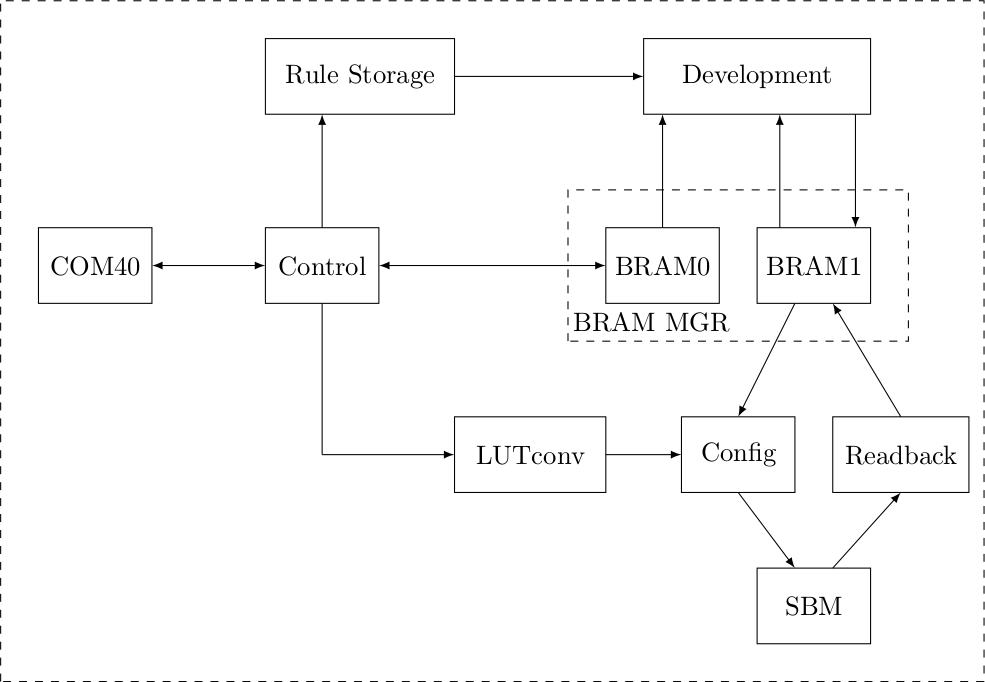
\includegraphics[width=0.5\textwidth]{figures/ca-djupdal}
    \caption{Original design by Djupdal (Reprinted from \cite{stovneng2014sblock})}
    \label{fig:ca-djupdal}
\end{figure}

\subsection{Extension: Aamodt \cite{aamodt2005sblock}}

\begin{itemize}
    \item Fig. \ref{fig:ca-aamodt}
\end{itemize}

\begin{figure}[!ht]
    \centering
    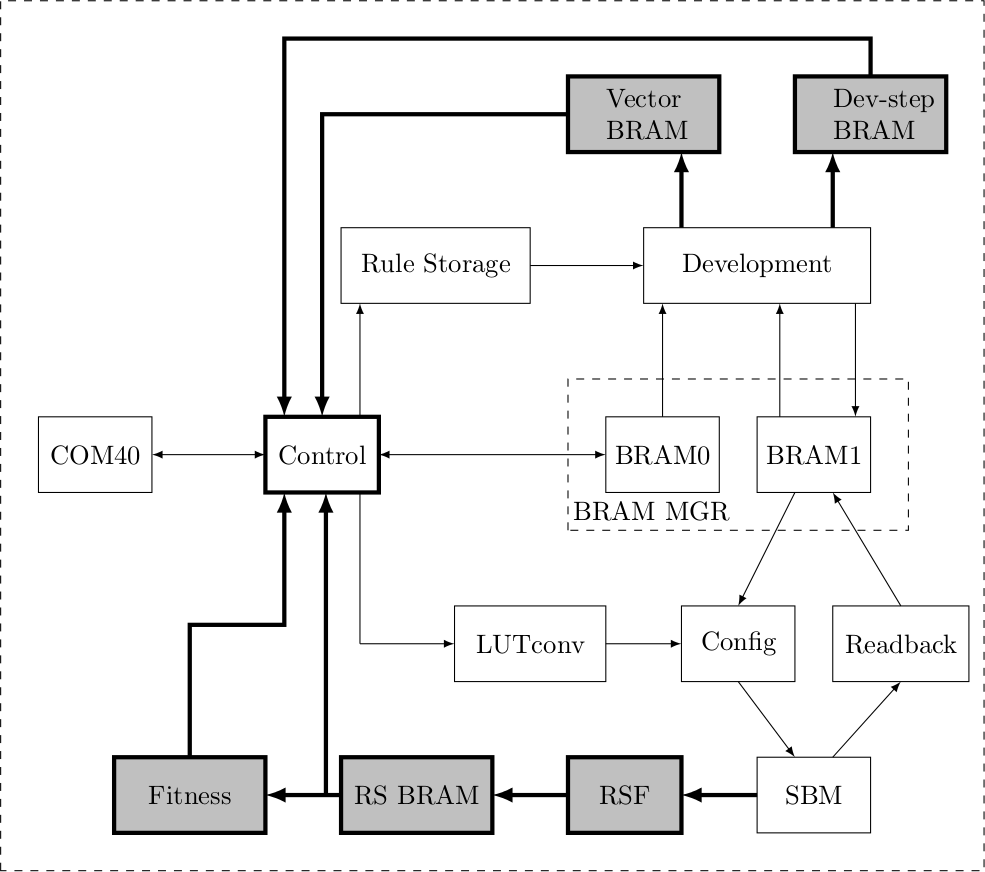
\includegraphics[width=0.5\textwidth]{figures/ca-aamodt}
    \caption{Additions by Aamodt (Reprinted from \cite{stovneng2014sblock})}
    \label{fig:ca-aamodt}
\end{figure}

\subsection{Renovation: Støvneng \cite{stovneng2014sblock}}

\begin{itemize}
    \item New hardware
    \item Fig. \ref{fig:ca-stovneng}
\end{itemize}

\begin{figure}[!ht]
    \centering
    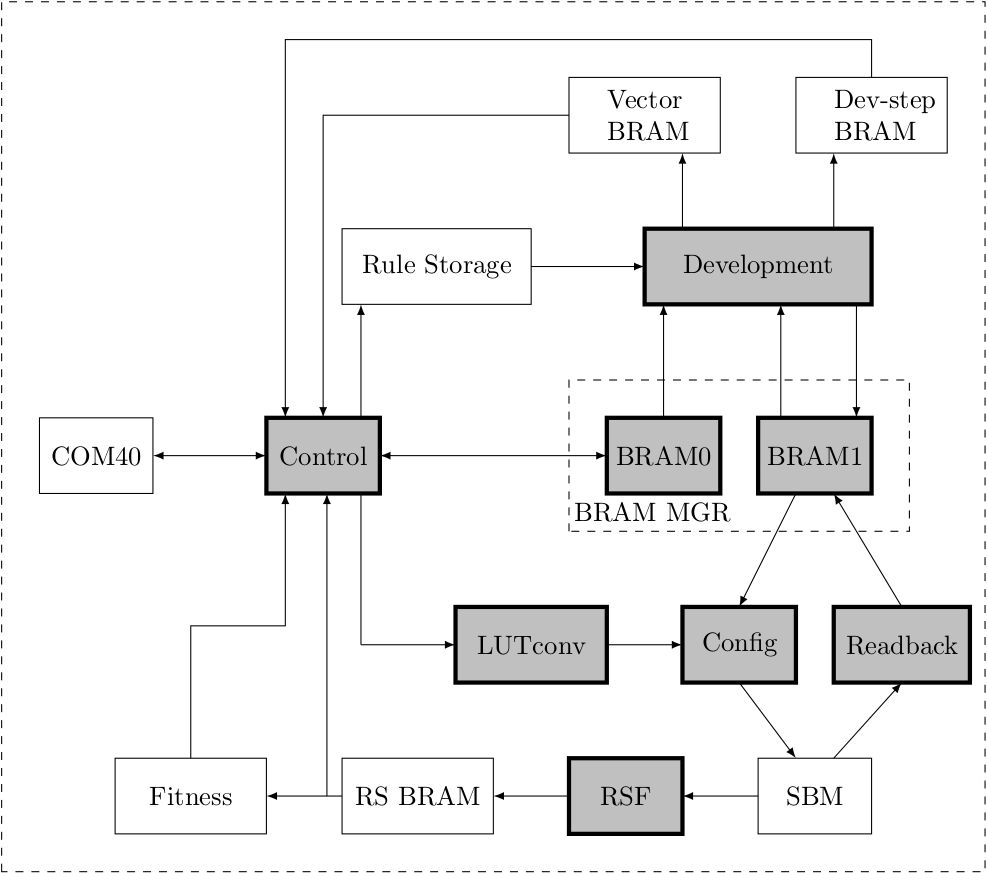
\includegraphics[width=0.5\textwidth]{figures/ca-stovneng}
    \caption{Parts optimized by Støvneng (Reprinted from \cite{stovneng2014sblock})}
    \label{fig:ca-stovneng}
\end{figure}

\todo{Tikz for diagrams: \url{http://www.texample.net/tikz/examples/noise-shaper/}}



\section{Communication}

    
Due to the difference in wordsize between the old and new communication unit, a compatibility layer is added to allow other existing code to remain unchanged.

\figurename~\ref{fig:overview-lundal} shows the changes to the hardware platform.
The old COM40 unit has been replaced by a new communication unit and a compatibility layer.
The compatibility layer is needed because the old COM40 unit was based on 64-bit data while PCI Express uses 32-bit data.
\todo{rewrite this}

\begin{figure}[!ht]
    \centering
    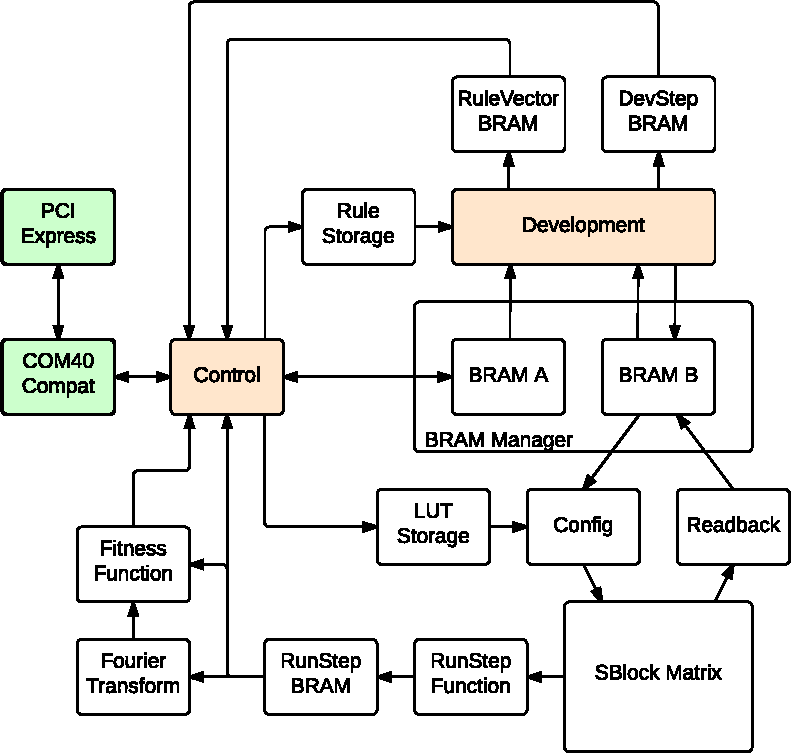
\includegraphics[width=0.48\textwidth]{figures/overview-lundal}
    \caption{High-level block diagram of the current hardware platform. Additions are highlighted in green.}
    \label{fig:overview-lundal}
\end{figure}

The communication unit has internal data buffers.

On the software side, the api uses linux' built-in drivers for PCI Express.

\subsection{Overview}

The new communication unit is based on Xilinx' reference PCI Express programmed io design.
It consists of the Xilinx PCI Express endpoint core, reception and transmission engines, data buffers, and a special request handler, as shown in \figurename~\ref{fig:details-communication}.

\begin{figure}[!ht]
    \centering
    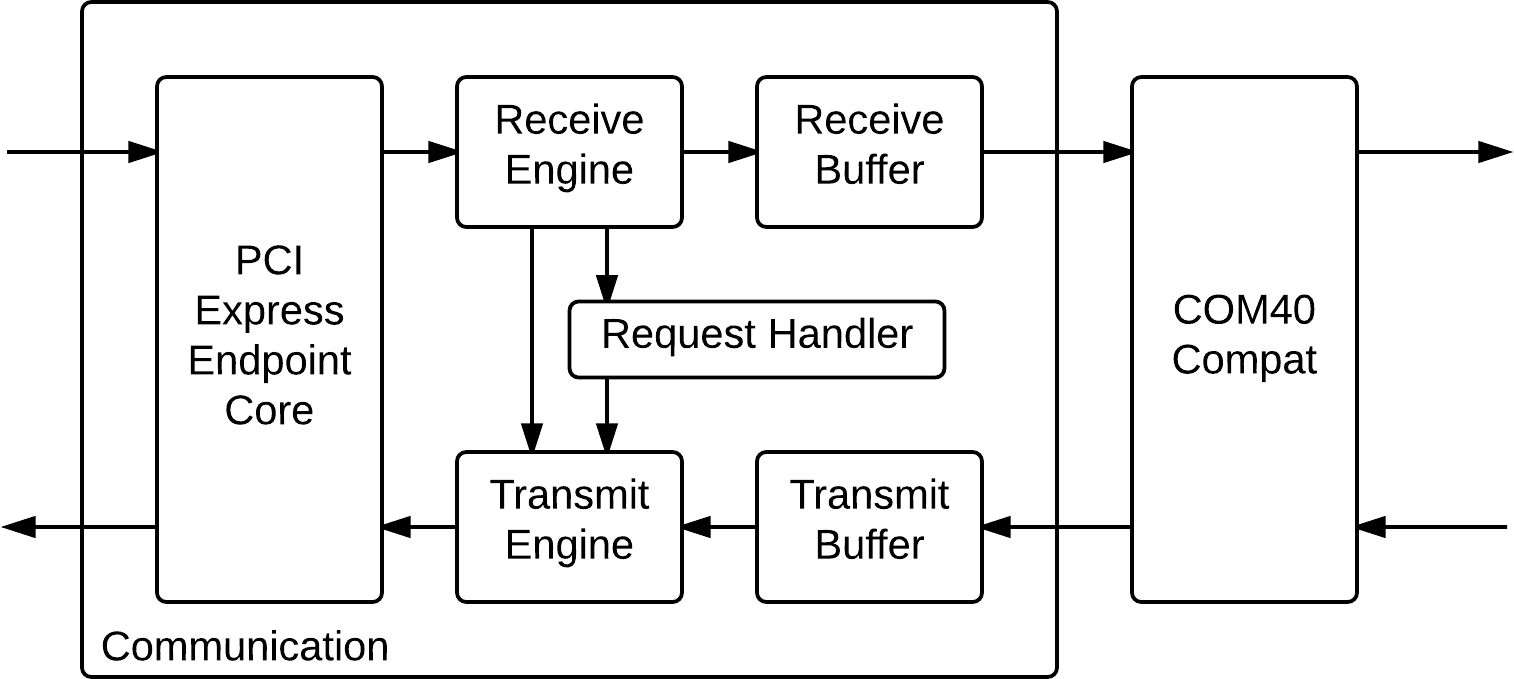
\includegraphics[width=0.48\textwidth]{figures/details-communication}
    \caption{Detailed block-diagram of the PCI Express communication module.}
    \label{fig:details-communication}
\end{figure}

The endpoint core completely handles the physical and data link layers, and all TLPs related to configuration and establishment of the PCI Express connection.
Other TLPs, such as read and write requests, are presented on an AXI4-Stream interface \cite{ug672}.
The reception engine is responsible for parsing TLPs and either writing received data to the reception buffer or notifying the transmission engine about a read request.
The transmission engine is responsible for building completer TLPs to respond to read requests, using data from the transmission buffer.
The request handler listens to the read requests provided by the reception engine, and can override the transmission engine to respond to special requests.

\subsection{PCI Express Endpoint Core}

\todo{bars, wrapper, id, more?}

\subsection{Reception engine}

The reception engine is implemented as a simple state machine, as shown in \figurename~\ref{fig:statemachine-receive}.

\begin{figure}[!ht]
    \centering
    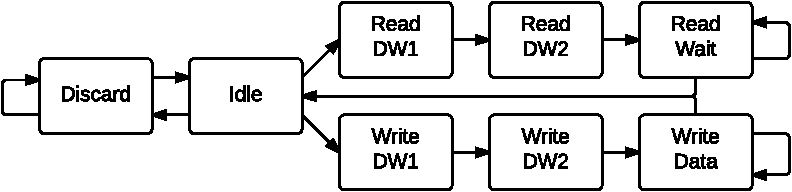
\includegraphics[width=0.48\textwidth]{figures/statemachine-receive}
    \caption{State machine for the reception engine.}
    \label{fig:statemachine-receive}
\end{figure}

Until the endpoint core presents valid data, the state machine remains in Idle.
When it does, the data is stored, and the TLP type is checked.
If it is a read or write request, the state machine continues down the corresponding path, otherwise the remaining data is discarded.
The remaining portion of the TLP headers are then parsed in the DW1 and DW2 states.
For read requests, the state machine waits in ReadWait until the transmission engine is ready to accept a new read request, and then proceeds to Idle.
For write requests, the state machine stays in WriteData, where one DW of data is written to the reception buffer each cycle, for the length of the packet, and then proceeds to Idle.

\subsection{Transmission engine}

The transmission engine is implemented as a simple state machine, as shown in \figurename~\ref{fig:statemachine-transmit}.

\begin{figure}[!ht]
    \centering
    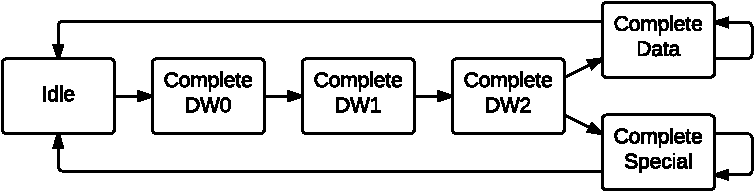
\includegraphics[width=0.48\textwidth]{figures/statemachine-transmit}
    \caption{State machine for the transmission engine.}
    \label{fig:statemachine-transmit}
\end{figure}

Until the reception engine signals a read request, the state machine remains in Idle.
When a read request is signaled by the reception engine, the state machine begins to traverse the DW path.
The DW0, DW1 and DW2 states each transmit one DW of the completer TLP header.
Then if the special request signal is set, it procceds to CompleteSpecial, where it transmits data presented by the request handler.
Otherwise, it proceeds to CompleteData where it transmits one DW of data from the transmission buffer each cycle.
When the requested number of DWs has been transmitted it proceeds back to Idle.

\subsection{Request handler}

The request handler continually listens to the read requests presented by the reception engine.
If the request is targeting the primary memory area (BAR 0), it is a normal read request and the transmission engine is allowed to proceed as usual.
Otherwise, it is a special request and the transmission engine is overridden.

The kind of special request is determined by the address of the read request, and handled thereafter.
There are currently four special requests implemented, as shown in Table~\ref{tab:requests}.

\begin{table}[!ht]
    \renewcommand{\arraystretch}{1.3}
    \caption{Special requests}
    \label{tab:requests}
    \centering
    \begin{tabular}{c|l}
        \bfseries Address & \bfseries Request \\
        \hline
        0x00 & Get transmission buffer data count \\
        0x01 & Get transmission buffer available space \\
        0x02 & Get reception buffer data count \\
        0x03 & Get reception buffer available space \\
    \end{tabular}
\end{table}

Note that each of the implemented special requests assumes a read request length of one DW.
If the request has a greater length, the returned data is simply repeated that number of times.

\subsection{Buffers}

\todo{describe fifo buffers}

\begin{figure}[!ht]
    \centering
    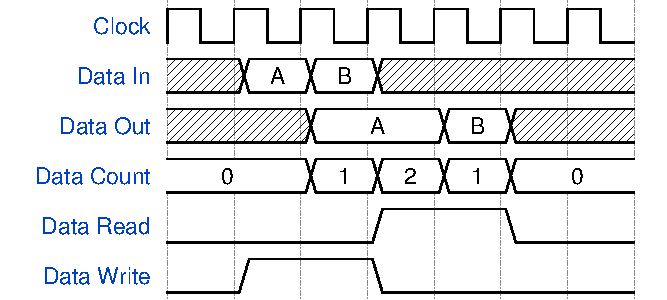
\includegraphics[width=0.40\textwidth]{figures/wavediagram-fifo}
    \caption{Wave diagram for the FIFO buffer, showing two consecutive writes followed by two consecutive reads.}
    \label{fig:wavediagram-fifo}
\end{figure}

Notice how the read signal needs to be asserted before the clock tick when data is read to ensure correct consecutive reads.
This is due to the BRAM used in the FIFO, which updates at clock ticks.
Therefore, the address has to be updated before the clock tick (by the read signal) to have correct data available for a read in the following cycle.

\subsection{Software API}

\todo{native linux driver, files under /sys/devices/pci}



\section{Testing}

    \todo{something about testing the com unit}

\todo{8x8, 8x8x8 matrices}

\todo{something about testbench}

Testing uncovered many bugs within the design

\subsection{Fixed issues}

\emph{States and types were written to the wrong location.}
When writing single states or types, a half-row is read from BRAM, combined with the new data, and written back to BRAM.
Due to the usage of non-implementable code to specify how the data should be combined, the new data always ended up in the middle of the half-row.

\emph{Development ran indefinitely.}
Comparison of signals of different widths always return false.
Due to the comparison of a parameterized signal with a constant, the development unit would not iterate through the cells, and thus never finish.

\emph{WriteRule did not follow spesification.}
When the api transformed a 3D rule struct into an instruction, the position of up/down and north/south were swapped.

\emph{PrintTypes used wrong offsets for decomposition.}
When decomposing a row of types into individual types, an offset of 5 was used instead of 8.
This entailed that the printed values were completely wrong.

\emph{ReadVector and PrintVector used 32-bit words.}
The functions were not updated from using 32-bit to 64-bit words.
ReadVector would therefore expect twice the number of words provided by the hardware platform, causing the program to wait for nonexistant data.

\subsection{Remaining issues}

\emph{ReadStates prints gargabe in top 32 bits.}
This occurs due to a buffering error in the LSS unit.
However, only the least 32 bits are used by the api, which means that this issue only impacts performance and not functionality.

\emph{WriteStates and WriteTypes does nothing in 3D.}
This issue is only present on the board, not in any simulations, which makes it hard to track down the cause.

\emph{ReadRuleVector sends incorrect data.}
The first execution of the instruction produces an extra word; a repetition of the first.
Following executions produces the correct amount of words, but the order is offset by one.

\emph{ReadUsedRules fails for SBM widths less than 16.}
The simulator crashes with an index-out-of-bounds error, due to the instruction accessing bit 63 of a signal that is $[width\cdot4]$ bits wide.
How ISE is able to implement the design despite illegal indexing is a mystery, but the instruction produces only zeroes on the board.

\emph{Development rules does not activate.}
This issue is also only present on the board, making it hard to analyze.
The root cause could be with any of the following instructions: devstep, writeRule and setNumberOfLastRule.

\emph{Config does not properly write states in 3D.}
Simulations show that the BRAM address fluctuates \TODO.

\emph{Runstep causes every state to become zero.}
\TODO

\subsection{Current status}

\TODO

\begin{itemize}
    \item PCIe com unit works beautifully
    \item Large parts are non-functional
\end{itemize}

\begin{table}[!ht]
    \renewcommand{\arraystretch}{1.3}
    \caption{Implementational status of instructions}
    \label{tab:instructions}
    \centering
    \begin{tabular}{l|l|l}
        \bfseries Instruction & \bfseries Works in 2D & \bfseries Works in 3D \\
        \hline
        break & Yes & Yes \\
        clearBRAM & Yes & Yes \\
        config & Yes & Undecidable \\
        devstep & Undecidable & Undecidable \\
        doFitness & Undecidable & Undecidable \\
        end & Yes & Yes \\
        jump & Yes & Yes \\
        jumpEqual & Yes & Yes \\
        nop & Yes & Yes \\
        readback & Yes & Undecidable \\
        readFitness & Undecidable & Undecidable \\
        readRuleVector & No & No \\
        readState & Yes & Yes \\
        readStates & Yes & Yes \\
        readSums & Undecidable & Undecidable \\
        readType & Yes & Yes \\
        readTypes & Yes & Yes \\
        readUsedRules & Undecidable & No \\
        resetDevCounter & Yes & Yes \\
        run & Undecidable & Undecidable \\
        setNumberOfLastRule & Undecidable & Undecidable \\
        startDFT & Undecidable & Undecidable \\
        store & Yes & Yes \\
        switch & Yes & Yes \\
        writeLUTConv & Undecidable & Undecidable \\
        writeRule & Undecidable & Undecidable \\
        writeState & Yes & Yes \\
        writeStates & Yes & No \\
        writeType & Yes & Yes \\
        writeTypes & Yes & No \\
    \end{tabular}
\end{table}



\section{Discussion}

    \todo{add section intro}

\subsection{Challenges}
\label{sec:challenges}

There was a lot of concern during initial hardware testing, as the SP605 was not detected by the computer.
A slightly curved circuit board led to the beilief that there might be something wrong with hardware.
Luckily, it proved not to be a hardware fault, but a mistake in the hardware setup guide; the position of SW1 was reversed, causing the board to operate in a completely different mode.

The SP605 was pre-installed with an example design implementing communication over PCI Express with DMA.
However, the accompanying driver did not support newer linux kernels.
Additionaly, the design was written in verilog while CARP is written in vhdl, which meant extra effort to integrate the two.
There was some effort applied to update the driver, but it was abandoned due to near-untraceable segfaults.

The USB cable driver for usage of JTAG provided by Xilinx also had the problem of not being compatible with newer linux kernels.
Thankfully, a the driver found at \cite{usbdriver} is compatible and solves the problem.

\todo{Development bug}

\begin{itemize}
    \item Works in post-translate sim
    \item Doesn't work on dev board
    \item All post-map and post-par simulations give X'es
    \item Can't keep\_hierarchy to trace source
\end{itemize}

\subsection{Future work}

The most important thing going forward is to fix the errors that are preventing the sblockmatrix and development units from working correctly.
However, this is no easy task, as large parts of the design are highly complex and difficult to debug.
The most extreme cases are the development and LSS units which each consists of a single large file, around 1200 lines long, of complex pipelined code.
Simplification and modularization of these units is therefore imperative.

Another reason to simplify the development unit is it's extreme memory bandwidth requirement against the SBM BRAM.
Currently, the it is designed so that N rules are loaded, applied to every cell, then the N next rules loaded and so on.
This means that the SBM BRAM must supply 5 rows each cycle to test 1 row per cycle (or 8 for 2) in 3D, while N rules are needed per matrix iteration.
In addition, after the first pass, cells has to be read from BRAM B instead of BRAM A, since some cells might have changed.

A simplified process would be to read 5 rows, apply one rule to the center row each cycle, then read the next 5 rows, and so on.
This will greatly lessen the bandwidth requirements against the SBM BRAM, as the rows can be read in sequence while each rule is being applied.
Assuming there are more rules than the number of rows that must be read (highly likely), there is no performance loss.
Additionally, this would allow development to only read from BRAM A.

There are still some remains of having two clock domains, more specificaly a pair of flipflops used for clock-synchronization in the fetch and lss units.
It does not affect functionality, and has therefore been of low priority, but it does add a slight delay between the communication unit and the fetch and lss units when reading data.

Currently, the platform only supports dimension sizes that are powers of 2.
It would be beneficial to be able to select any size, allowing for fine-tuning of the resource usage, to get most out of the FPGA.

As noted in \cite{stovneng2014sblock}, Støvneng increased the base instruction and data sizes from 32 to 64 bits.
Although it is one way to accomodate for longer instructions, the decision is a little odd, considering both PCI and PCI Express are based on 32-bit word sizes.
This means that conversion is currently required between the LSS and communication units.
Since only 6 out of 30 instructions require more than 32 bits, communication could be simplified and optimized by going back to a 32-bit base size.

Finally, a unification of the 2D and 3D designs would be \TODO

\begin{itemize}
    \item Com buffer checks
    \item Get rid of tristate buffers \cite{koch2008buses}
    \item Get rid of reset (init values in \cite{ug687} page 55-56, \cite{wp272} page 5)
    \item Use generics instead of global constants
    \item Unify 2D and 3D designs
    \item Add instruction that reports info (2D/3D, SIZE, ++)
    \item Add general purpose counters
    \item DMA (better performance?)
    \item Toggle SBM wrap-around
\end{itemize}

With the current need for major fixes, simplification of development and LSS, reducing the need for extreme memory bandwidth, removing tristates, removing resets, and unification, it might be a good idea to rebuild the platform from the ground up.
Starting from a clean slate, thoroughly evaluating every part of the design, replacing the bad features and improving the good, will likely result in a greatly improved platform for CA research.



\section{Future Work}

    The most important thing going forward is to fix the errors that are preventing the sblockmatrix and development units from working correctly.
However, this is no easy task, as large parts of the design are highly complex and difficult to debug.
The most extreme cases are the development and lss units which each consists of a single large file, around 1200 lines long, of complex pipelined code.
Simplification and modularization of these units is therefore imperative.

Another reason to simplify the development unit is it's extreme memory bandwidth requirement against the SBM BRAM.
Currently, the it is designed so that N rules are loaded, applied to every cell, then the N next rules loaded and so on.
This means that the SBM BRAM must supply 5 rows each cycle to test 1 row per cycle (or 8 for 2) in 3D, while N rules are needed per matrix iteration.
In addition, after the first pass, cells has to be read from BRAM B instead of BRAM A, since some cells might have changed.

A simplified process would be to read 5 rows, apply one rule to the center row each cycle, then read the next 5 rows, and so on.
This will greatly lessen the bandwidth requirements against the SBM BRAM, as the rows can be read in sequence while each rule is being applied.
Assuming there are more rules than the number of rows that must be read (highly likely), there is no performance loss.
Additionally, this would allow development to only read from BRAM A.

There are still some remains of having two clock domains, more specificaly a pair of flipflops used for clock-synchronization in the fetch and lss units.
It does not affect functionality, and has therefore been of low priority, but it does add a slight delay between the communication unit and the fetch and lss units when reading data.

Currently, the platform only supports dimension sizes that are powers of 2.
It would be beneficial to be able to select any size, allowing for fine-tuning of the resource usage, to get most out of the FPGA.

As noted in \cite{stovneng2014sblock}, Støvneng increased the base instruction and data sizes from 32 to 64 bits.
While it made sense to do so at the time to accomodate for longer instructions and optimize for the 64-bit PCI bus, PCI Express is based on a 32-bit word size, which means conversion is currently required.
Since only 6 out of 30 instructions require more than 32 bits, communication could be simplified and optimized by going back to a 32-bit base size.


Finally, a unification of the 2D and 3D designs would be \TODO

With the current need for major fixes, simplification of development and lss, reducing the need for extreme memory bandwidth, removing tristates, removing resets, and unification, it might be a good idea to rebuild the platform from the ground up.
Starting from a clean slate \TODO

\begin{itemize}
    \item Com buffer checks
    \item Get rid of tristate buffers \cite{koch2008buses}
    \item Get rid of reset (init values in \cite{ug687} page 55-56, \cite{wp272} page 5)
    \item Use generics instead of global constants
    \item Unify 2D and 3D designs
    \item Add instruction that reports info (2D/3D, SIZE, ++)
    \item Add general purpose counters
\end{itemize}

\subsection{Maybe}

\begin{itemize}
    \item DMA (better performance?)
    \item Toggle SBM wrap-around
\end{itemize}



\section{Conclusion}

\TODO

\bibliographystyle{IEEEtran}
\bibliography{IEEEabrv,bibliography}

\end{document}

